\section{Обзор существующих решений}
\label{sec:Chapter2} \index{Chapter2}

Одним из способов модификации программы является изменение ее семантики посредством рефлексии \cite{compReflection}, однако многие языки, в том числе $Java$ не предоставляют поддрежки для изменения семантики программы. Например, в $Java$ класс $Class$ объявлен $final$, что предотвращает специализацию данного класса с целью изменения семантики языковых механизмов, как это например возможно в $SmallTalk$. Исходя из этого, необходимо либо вносить изменения на уровне виртуальной машины, принося в жертву портабельность (как например делают мета-объектные протоколы ($Meta~Object~Protocol,~MOP$) $Metaxa$, $IguanaJ$), либо вносить изменения на уровне бинарного кода. Любые изменения исходного кода не рассматриваются, т.к. зачастую к нему нет доступа. Именно поэтому было сделано множество различных предложений по трансформации байткода, отличающихся по уровню абстракции сущностей, с которыми работает пользователь, по выразительной мощности и по гранулярности разрешенных преобразований.

В текущей главе будут рассмотрены существующие решения для решения задачи бинарной манипуляции, а также будет проведен анализ этих решений с точки зрения их области применения и архитектуры: какие из описанных во введении задач бинарной манипуляции они решают и каким образом интергируются в потребительские приложения.

\subsection{java.lang.classfile}

\cite{lavaLangClassfile}

\subsection{BIT}

Архитектура фреймворка $BIT$ основана на наблюдении, что для достижения большей части необходимых изменений достаточно инструментации только очень ограниченного количества ключевых локаций, таких как пролог и эпило функции, начало и конец базового блока, а также до и после конкретной инструкции. Поэтому $BIT$ предоставляет интерфейс для вызова методов в каждой из этих ключевых точек \cite{bit}. Как видно из описания, данный фреймвор работает с абстракциями бинарного файла, что дает возможность увеличить гранулярность инструментации.

\begin{figure}[h]
\centering
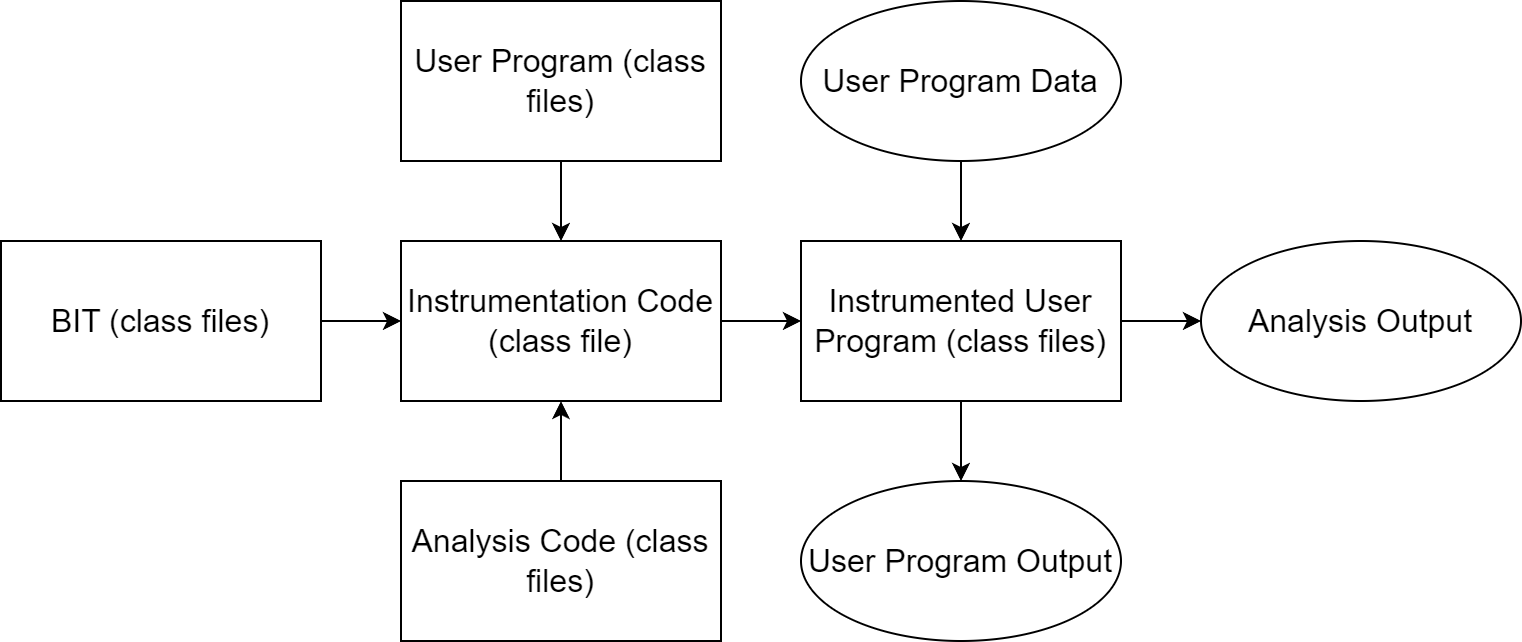
\includegraphics[width=.9\textwidth]{bit.png}
\caption{Архитектура фреймворка $BIT$.}
\label{fig:bitArch}
\end{figure}

На \autoref{fig:bitArch} проиллюстрирован процесс использования фреймворка $BIT$. Сначала пользователь пишет приложение, которое в последствии захочет инструментировать. Затем он пишет непосредственно код для инструментации и код для анализа бинарных файлов, используя классы и методы, предоставляемые фреймворком. Когда пользователь запустит код для инструментации, виртуальной машиной будут считаны бинарные файлы пользовательского приложения, после чего в нужные места пользовательского приложения будут вставлены вызовы кода для анализа. В результате получится инструментированное приложение, которое может впоследствии быть исполнено виртуальной машиной $Java$. Исполнение инструментированного приложения порождает как вывод оригинальной пользовательской программы, так и вывод анализа. Вставленные вызовы к функциям анализа ни коим образом не влияют на семантику приложения, и его вывод должен остаться неизменным.

Таким образом, $BIT$ - это инструмент для создания специализированных инструментов для наблюдения и анализа поведения программ во время исполнения. $BIT$ позволяет пользователям добавлять производить анализ в любом месте бинарного кода, а также получать динамическую информацию о программе во время исполнения. Подобные возможности делают $BIT$ хорошим вариантом для имплементации профилировщиков и других схожих инструментов.

Ниже приведен пример того, как выглядит инструментация на фреймворке $BIT$. В \autoref{lst:Instrumentation} и \autoref{lst:Analysis} показано, каким образом будет выглядеть код для подсчета условных переходов во время исполнения.

\begin{lstlisting}[language=Java, caption=Подсчет условных переходов на $BIT$. Код инструментации, label=lst:Instrumentation]
// filenameIn = ...; filenameOut = ...;
ClassInfo ci = new ClassInfo(filenameIn);
for (Enumeration e=ci.getRoutines().elements();e.hasMoreElements(); ){
    Routine routine = (Routine) e.nextElement();
    Vector instructions = routine.getInstructions();
    for (Enumeration b = routine.getBasicBlocks().elements(); b.hasMoreElements(); ) {
        BasicBlock bb = (BasicBlock) b.nextElement();
        Instruction instr = (Instruction)instructions.elementAt(bb.getEndAddress());
        short instr_type = InstructionTable.InstructionTypeTable[instr.getOpcode()];
        if (instr_type == InstructionTable.CONDITIONAL_INSTRUCTION) {
            instr.addBefore("BranchPrediction", "Offset", new Integer(instr.getOrigOffset()));
            instr.addBefore("BranchPrediction", "Branch", new String("BranchOutcome"));
        }
    }
    String method = new String(routine.getMethod());
    routine.addBefore("BranchPrediction", "EnterMethod", method);
    routine.addAfter("BranchPrediction", "LeaveMethod", method);
}
ci.write(filenameOut);
\end{lstlisting}

Заметим, что методы $addBefore$ и $addAfter$ добавляют вызовы к функциям, объявлены пользователем в коде анализа \autoref{lst:Analysis}.

\begin{lstlisting}[language=Java, caption=Подсчет условных переходов на $BIT$. Код анализа, label=lst:Analysis]
public BranchPrediction {
    static Hashtable branch = null;
    static int pc = 0;
    public static void EnterMethod(String s) {
        branch = new Hashtable();
    }
    public static void LeaveMethod(String s) {
        System.out.println("stat for method: " + s);
        for (Enumeration e = branch.keys(); e.hasMoreElements(); ) {
            // Log results
        }
    }
    public static void Offset(int offset) {
        pc = offset;
    }
    public static void Branch(int brOutcome) {
        Branch b = (Branch) branch.get(pc);
        if (b == null)
            b = new Branch();
        if (brOutcome == 0)
            b.taken++;
        else
            b.not_taken++;
    }
}
\end{lstlisting}

\subsection{BCA}

\cite{bca}


There are several general-purpose implementations of bytecode manipulation
available: BCEL [21], JikesBT [22], and JOIE [23]. All of them translate the
class file data structure into an intermediate representation, allow the user to
perform modifications and to finally regenerate a valid class file data structure
from the transformed intermediate representation. The bytecode-level API of
Javassist [11] could fit into this category although bytecode instructions are not
reified: the programmer is just provided with an iterator over a sequence of
bytes. The main strength of these general-purpose extensions is their expressive
power, since they are able to express anything that can be written in bytecode.
However, their main drawback is to be low-level and therefore difficult to use.

\subsection{BCEL}

% \cite{bcel}

\subsection{Kava}

Примером фреймворка, расширящего стандартные средства рефлексии языка является $Kava$ \cite{kava1} \cite{kava2}. Большинство фреймворков для манипуляции байткодом предоставляют объектно-ориентированное представление для элементов бинарного класс-файла таких как методы, типы, инструкции и других. После чего пользователю предлагается написать отдельную программу, описывающую, как переписать класс файл. Главным недостатком данного подхода является то, что для того чтобы им возпользоваться, пользователь должен обладать знаниями о байткода и формате бинарного файла платформы. Альтернативныс является подход, оперирующий на языковом уровне, что несколько обезопасит и облегчит использование программистом бинарного кода. Поэтому $Kava$ предлагает модель на основе поведенческой рефлексии, позволяющая изменять поведение приложения без необходимости изменения имплементации всей программы.

Для представления языковых сущностей $Kava$ использует метаобъекты ($Meta~Object~Protocol$). При их помощи поведение сущностей во время исполнения, например доступ к полю, вызов метода и другие, могут быть переопределены. Метаобъекты конструируются при помощи овеществления (reification) рантайм модели объектов. Например, метод овеществляется как объект класса $Method$.

\begin{figure}[h]
\centering
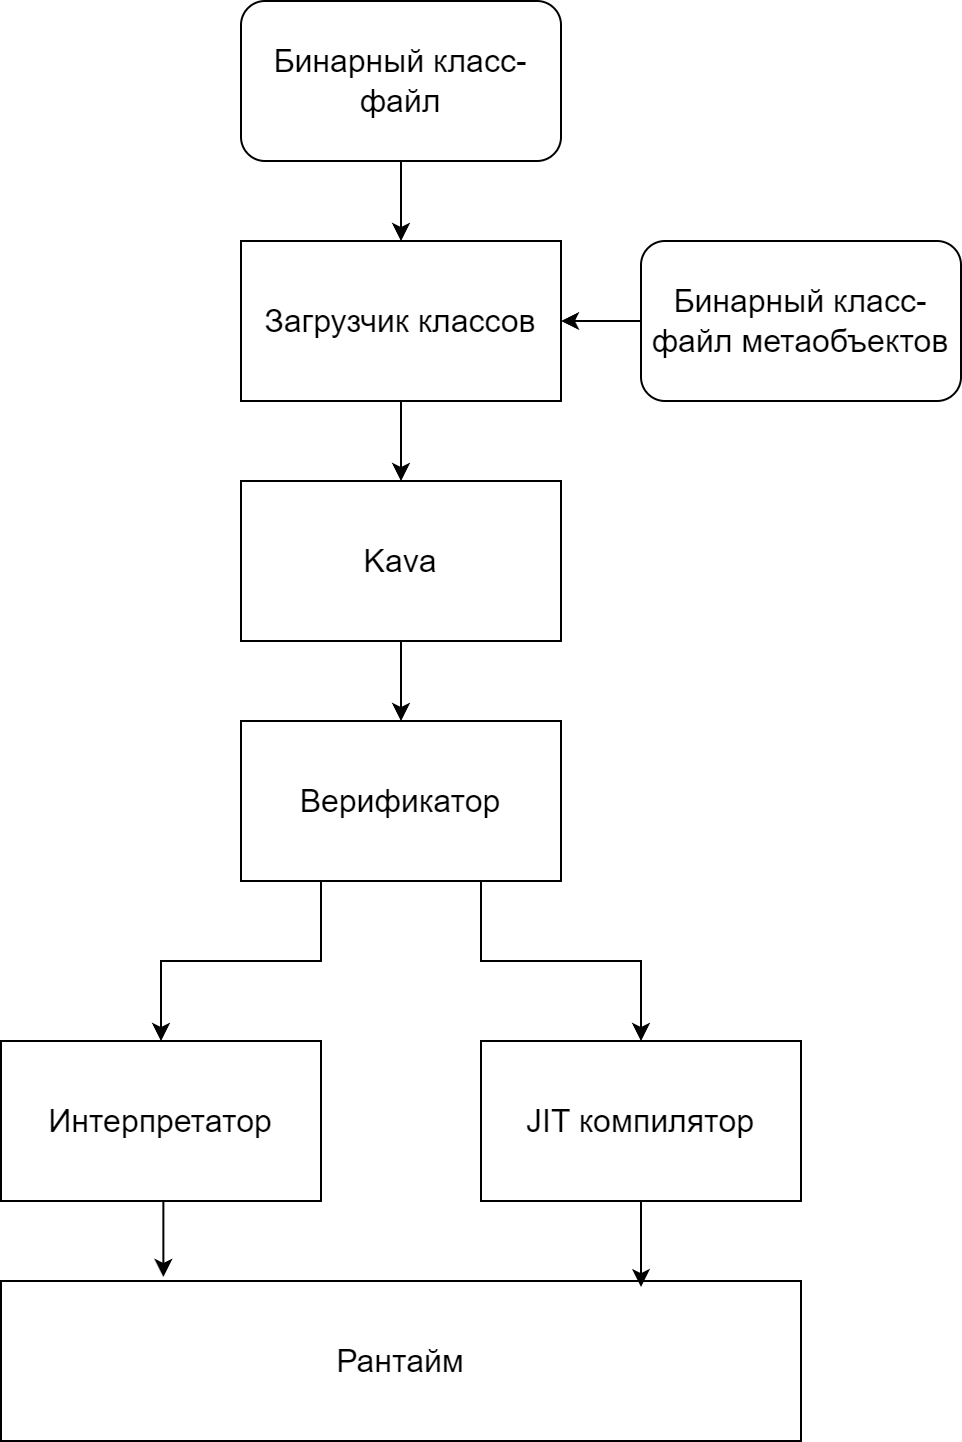
\includegraphics[width=.5\textwidth]{kava.png}
\caption{Архитектура фреймворка $Kava$.}
\label{fig:kavaArch}
\end{figure}

Как видно из \autoref{fig:kavaArch}, $Kava$ реализована при помощи инструментирования класс файла кодом, передающим контроль метаобъекту, ассоциированному с объектом. Для манипуляции самим байткодом $Kava$ использует сторонний низкоуровневый фреймворк $BCEL$. При помощи него $Kava$ инструментирует класс-файл во время его загрузки, что позволяет пользователю перехватывать и переопределять такие события как доступ к полю класса, вызов метода, вызов конструктора или выброс программой исключения.

Ниже в \autoref{lst:kava1} представлен простой пример работы с $Kava$. В нем пользователь хочет перехватить исполнение метода, пожтому он переопределяет процесс исполнения функций платформой, исполняющей $Java$. Перед исполнением функции будут выведены ее имя и дополнительная информация.

\begin{lstlisting}[language=Java, caption=Объявление метаобъекта в $Kava$, label=lst:kava1]
public class TracingMetaObject implements MetaObject {
    public ExecutionContext beforeExecuteMethod(ExecutionContext context) {
        System.out.println("tracing " + context.getMethodName());
    }
};
\end{lstlisting}

Для достижения желаемого результата, метаобъект должен быть привязан к классу, вызов методов которого необходимо отслеживать. Код, приведенный в \autoref{lst:kava2}, показывает как добиться отслеживания вызовов всех методов класса $Test$.

\begin{lstlisting}[language=Java, caption=Привязка класса к метаобъекту в $Kava$, label=lst:kava2]
bind {
    class Test metaclass-is TracingMetaObject {
        any-method(any-parameters) {
            execute;
        }
    }
}
\end{lstlisting}

Для сравнения, имплементация эквивалентной логики при помощи классического фреймворка для работы с класс-файлами приведен ниже в \autoref{lst:kava3}

\begin{lstlisting}[language=Java, caption=Реализация аналогичной функциональности при помощи классического фреймворка для работы с класс-файлом, label=lst:kava3]
public class TraceMethod implements Constants {
    private static Method traceMethod(Method m) {
        // create the byte code to insert
        // find insertion point
        // insert byte code at beginning of method
        // recalculate stack size
        // return modified method
    }
    public static void main(String[] argv) {
        // parse the class
        // get constant pool
        // generate necessary constants
        // foreach method:
        // call traceMethod
        // write out modified class
    }
}
\end{lstlisting}

У данного подхода есть несколько недостатков в сравнении с реализацией через расширенный механизм рефлексии. Во первых, программист должен самостоятельно генерировать инструкции, которые необходимо вставить в бинарное представление методов, а также самостоятельно обходить класс-файл чтобы найти нужную точку вставки нового кода. Вдобавок, вставленный код может быть верифицирован только при повторной загрузке класс-файла. При помощи расширения механизма рефлексии бинарной манипуляцией, этих недостатков удается избежать.

\subsection{AspectJ}

\cite{aspectj}

\subsection{Javassist}

\cite{javassist}

\subsection{ASM}

\cite{asm}

Здесь надо рассмотреть все существующие решения поставленной задачи, но не
просто пересказать, в чем там дело, а оценить степень их соответствия тем
ограничениям, которые были сформулированы в постановке задачи.

\newpage
